%
\documentclass[english]{article}
%%%%%%%%%%%%%%%%%%%%%%%%%%%%%%%%%%%%%%%%%%%%%%%%%%%%%%%%%%%%%%%%%%%%%%%%%%%%%%%%%%%%%%%%%%%%%%%%%%%%%%%%%%%%%%%%%%%%%%%%%%%%
\usepackage{latexsym,amsmath,amssymb,amsfonts,fullpage,graphicx,placeins}
\usepackage[capposition=top]{floatrow}

\begin{document}
Gabrielle Merritt 
\\
gmerritt@seas.upenn.edu 
\begin{center}
{\textbf{ESE 505 Homework 3}} \\

\end{center}

\section{Step Response}
Below is a picture of the step response for the transfer function described in the homework 
$$
\frac{2a^3}{s^3+3as^2 + 3a^2s+ a^3}
$$
\begin{figure}[h!]
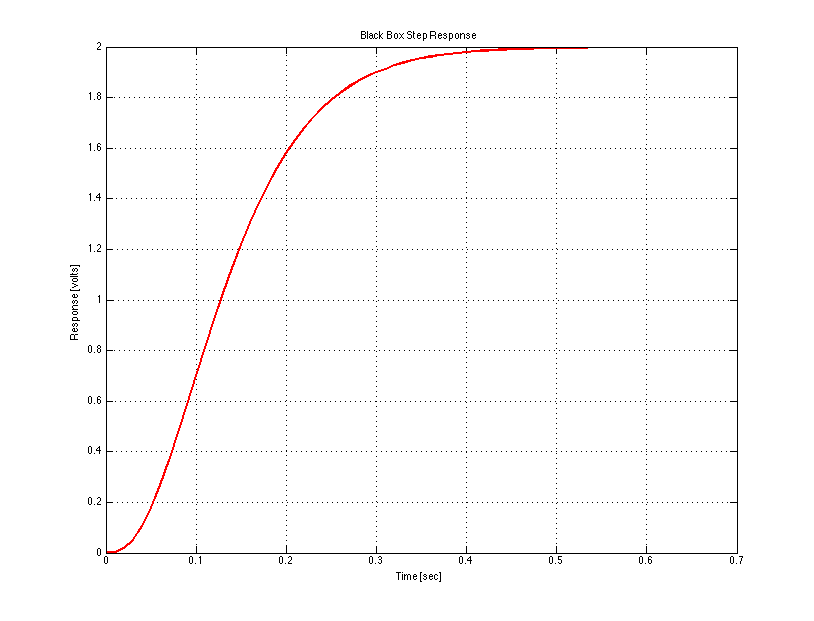
\includegraphics[width = \linewidth]{blackbox_step_graph1.png}
\caption{Step response }
\floatfoot{generated using Matlab built in transfer funcition} 
\end{figure}
\FloatBarrier 

\begin{figure}[h!]
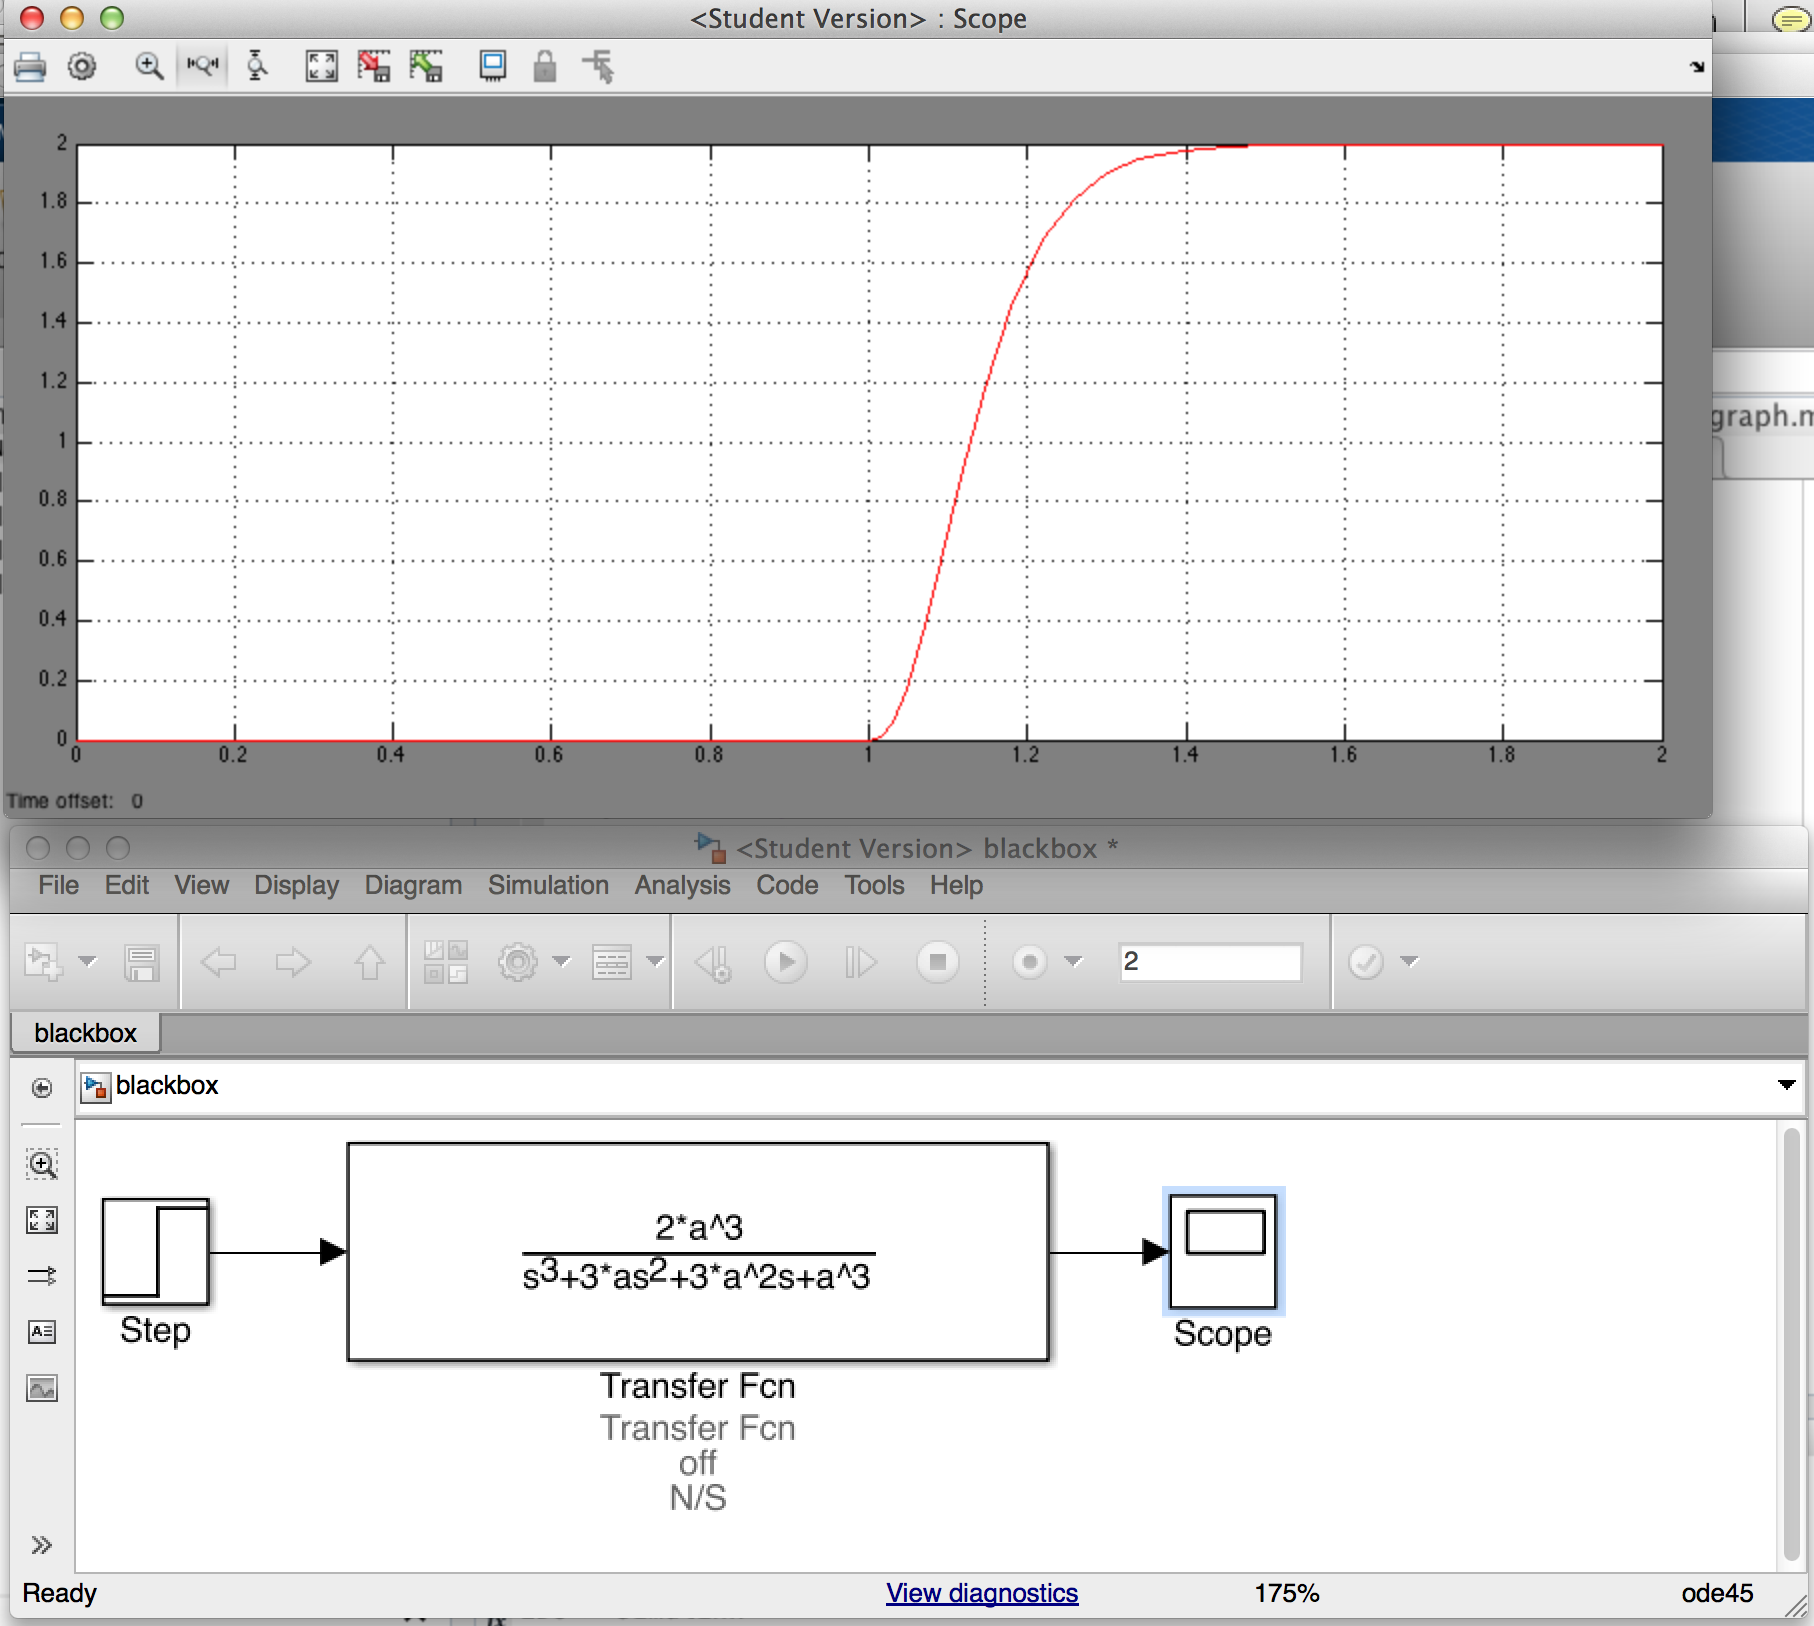
\includegraphics[width = \linewidth]{simlink1.png}
\caption{Simulink step response}
\floatfoot{Generated using Simulink model} 
\end{figure}
\FloatBarrier

\begin{figure}[h!]
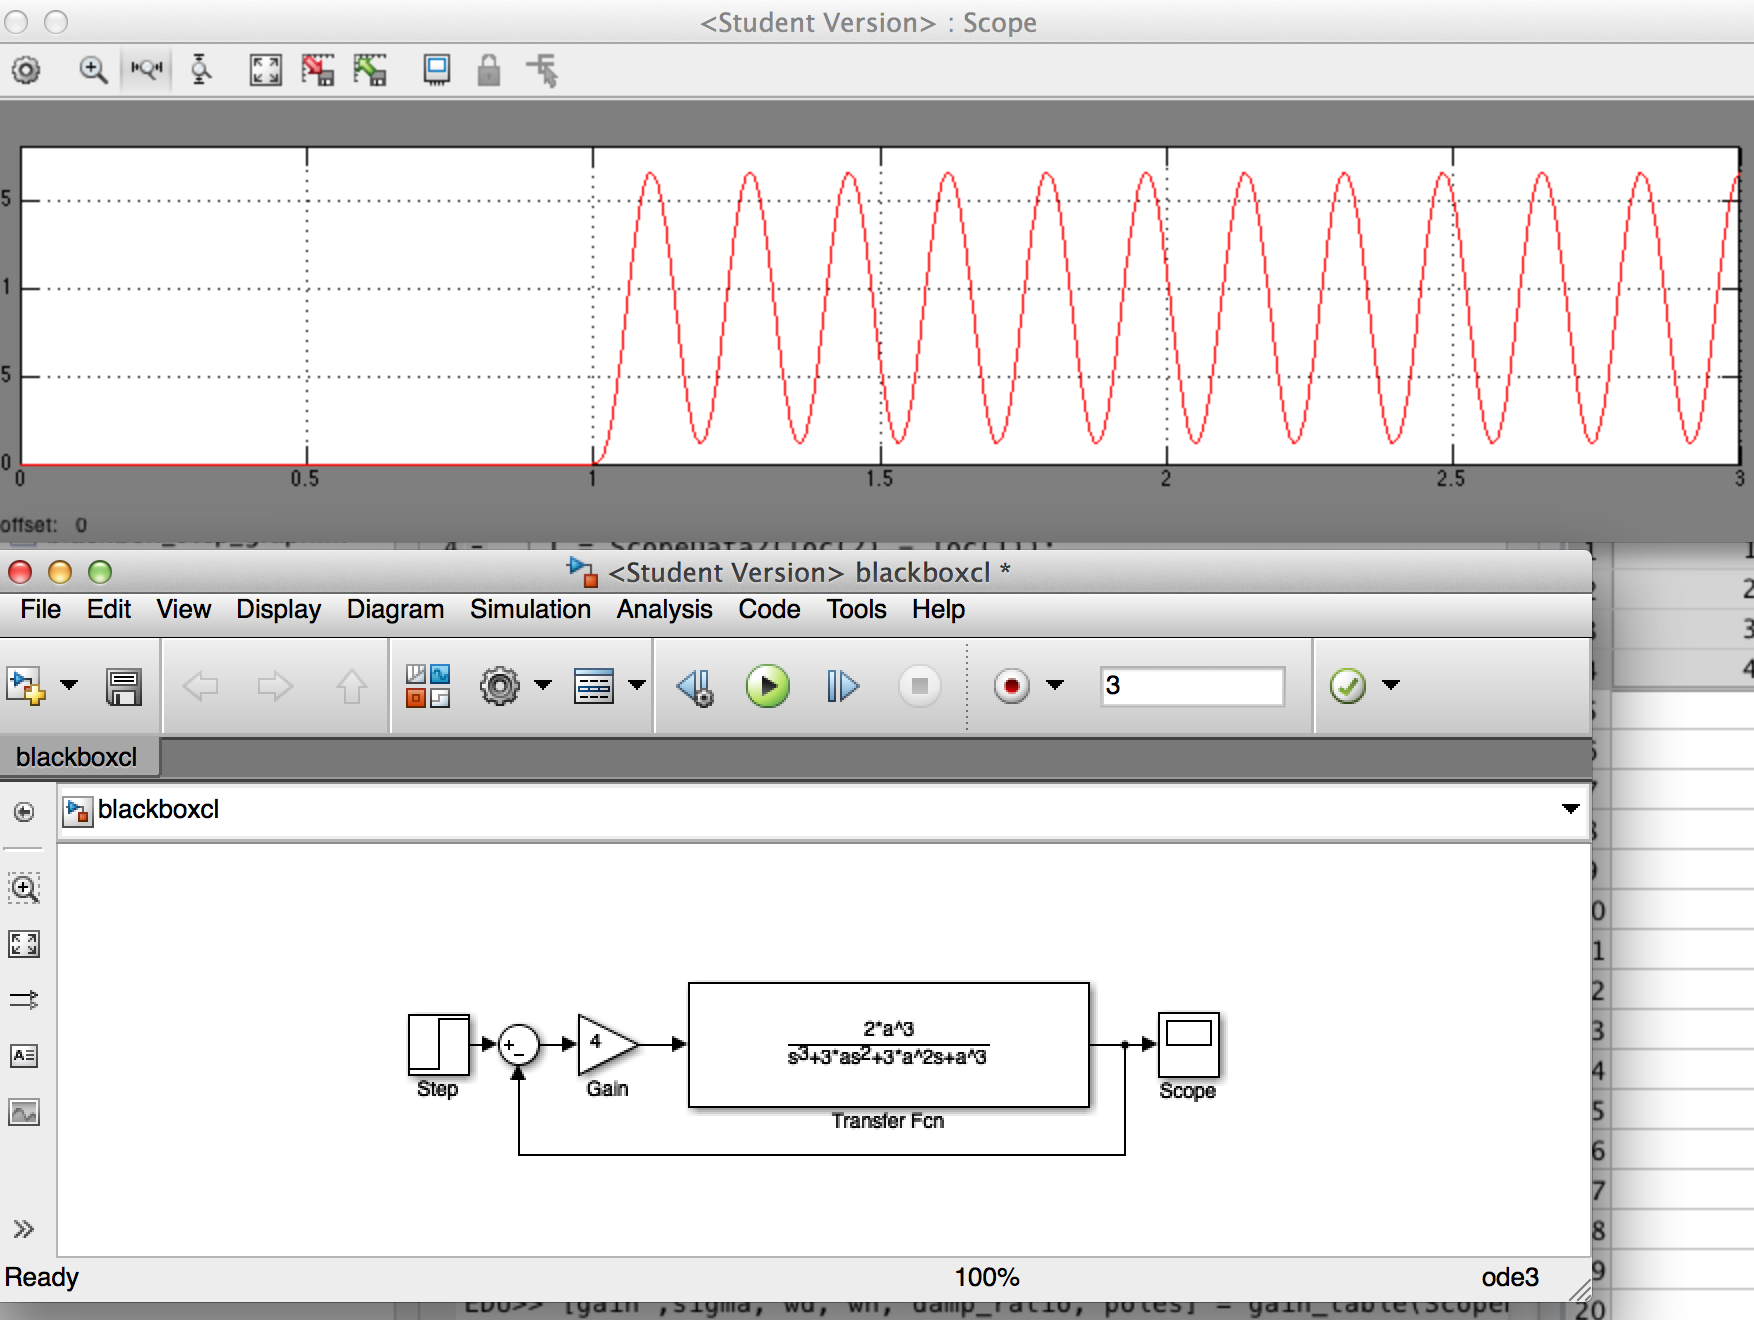
\includegraphics[width = \linewidth]{simulink2.png}
\caption{Simulink Proportional Gain (K =4)}
\floatfoot{Generated using Simulink model} 
\end{figure}

\FloatBarrier
\section{Root Locus and Poles}
\begin{table}[h]
\begin{tabular}{|l|l|l|l|l|}
K & $\sigma $&$ \omega_d$ &$ \omega_n $&$ \zeta$ \\
1 & -7.7756 & 22.9313 & 24.2138 & 0.3211        \\
2 & -4.324  & 28.822  & 29.1446 & 0.14838       \\
3 & -1.9209 & 33.069  & 33.1251 & 0.05799       \\
4 & 0.0010  & 36.319  & 36.319  & -2.788021e-05
\end{tabular}
\end{table}
\begin{figure}[h!]
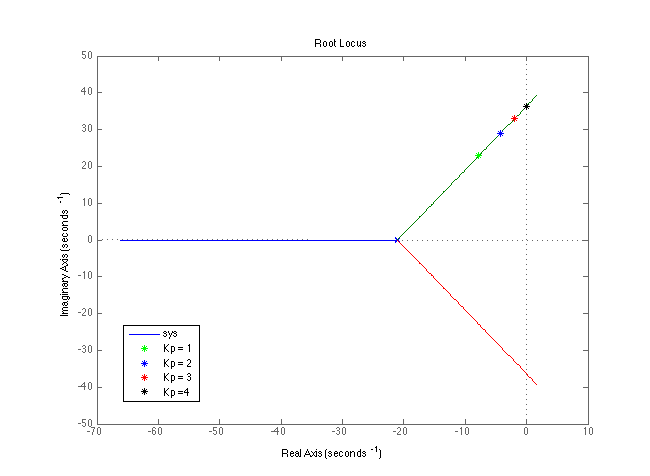
\includegraphics[width = \linewidth]{rlocus_kp.png}
\caption{Root Locus for Transfer Function}
\floatfoot{Using different Gains to see effect on pole position} 
\end{figure}
\FloatBarrier

\section{Closed loop control with Derivative Gain}
Kd = .0257   
To obtain this I used the damping ratio from my table as as well as my natural frequency to find kd. 
I found Kd using sgrid and rlocfind. S grid to locate the point on the root locust curve that corresponded to damping my proportional gains. I noticed that it is slightly off from the recommended gain of .0257, I think this is due to some errors I might have in finding my damping ratio. 
\begin{figure}[h!]
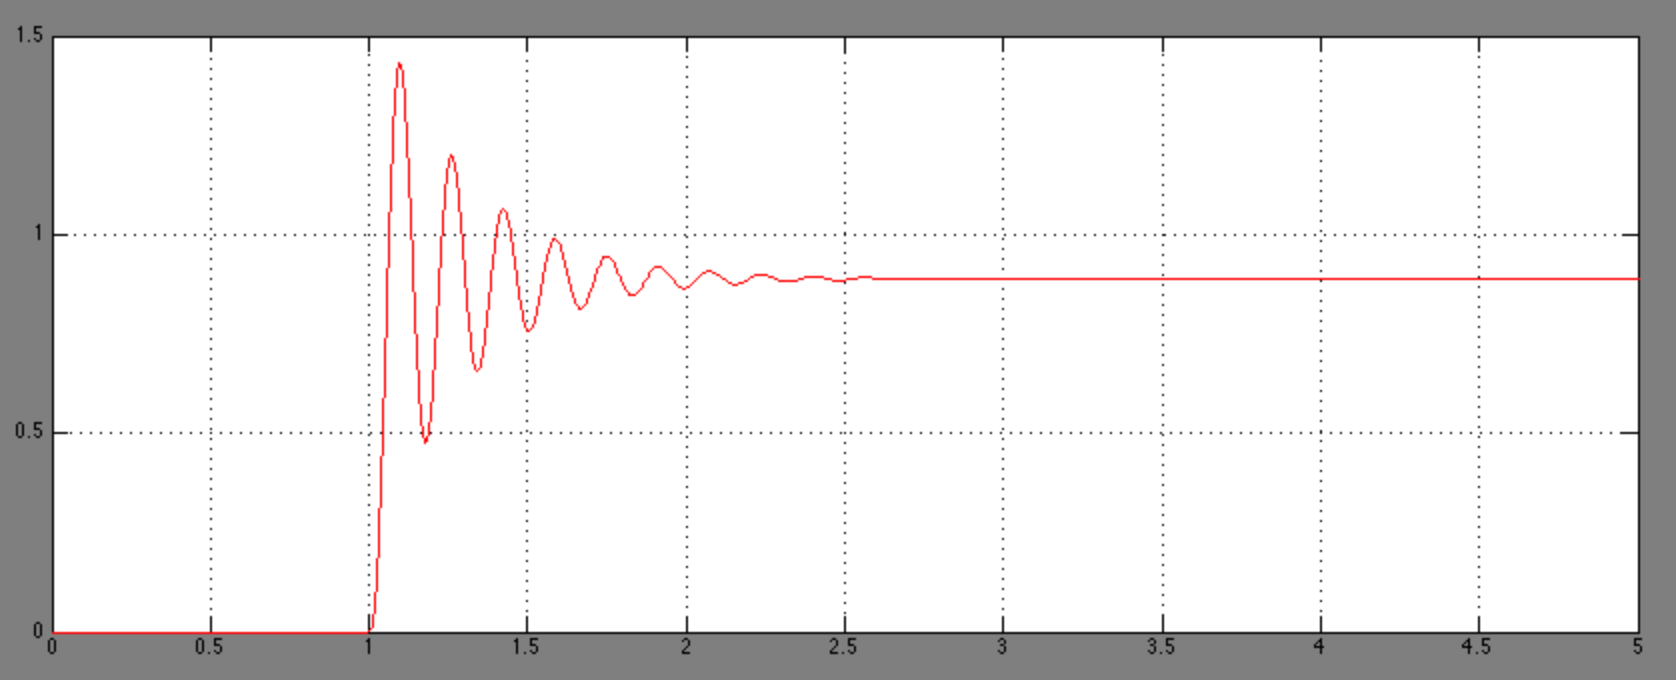
\includegraphics[width = \linewidth]{sim3.png}
\caption{Simulink Proportional Gain (K =4) and Derivative Gain (Kd = .0257) }
\floatfoot{Generated using Simulink model} 
\end{figure}
\FloatBarrier


\section{Adding an Integral Term}
Initial damp ratio  $ = .0904$ with$ K_I$ set to  0.  
For this part of the assignment I used the form 
$$ D_p + K_pN(s) + sK_dN(s) + \frac{1}{s}K_IN(S) = 0 
$$ 
Where 
$$ A(s) = D_P + s^2K_dN(s) + sK_pN(s) $$ 
$$ B(s) = N(s) $$

After generating a range of $K_I$ values  I go this root locus graph
\begin{figure}[h!]
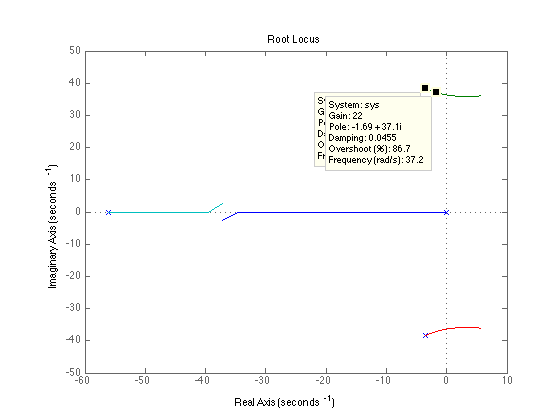
\includegraphics[width = \linewidth]{rlocus_ki.png}
\caption{PID transfer function}
\floatfoot{Generated using Transfer function} 
\end{figure}
\FloatBarrier 

I was able to extract a $K_I$ of $22$  and a damping constant of $.0455$ 
\begin{figure}[h!]
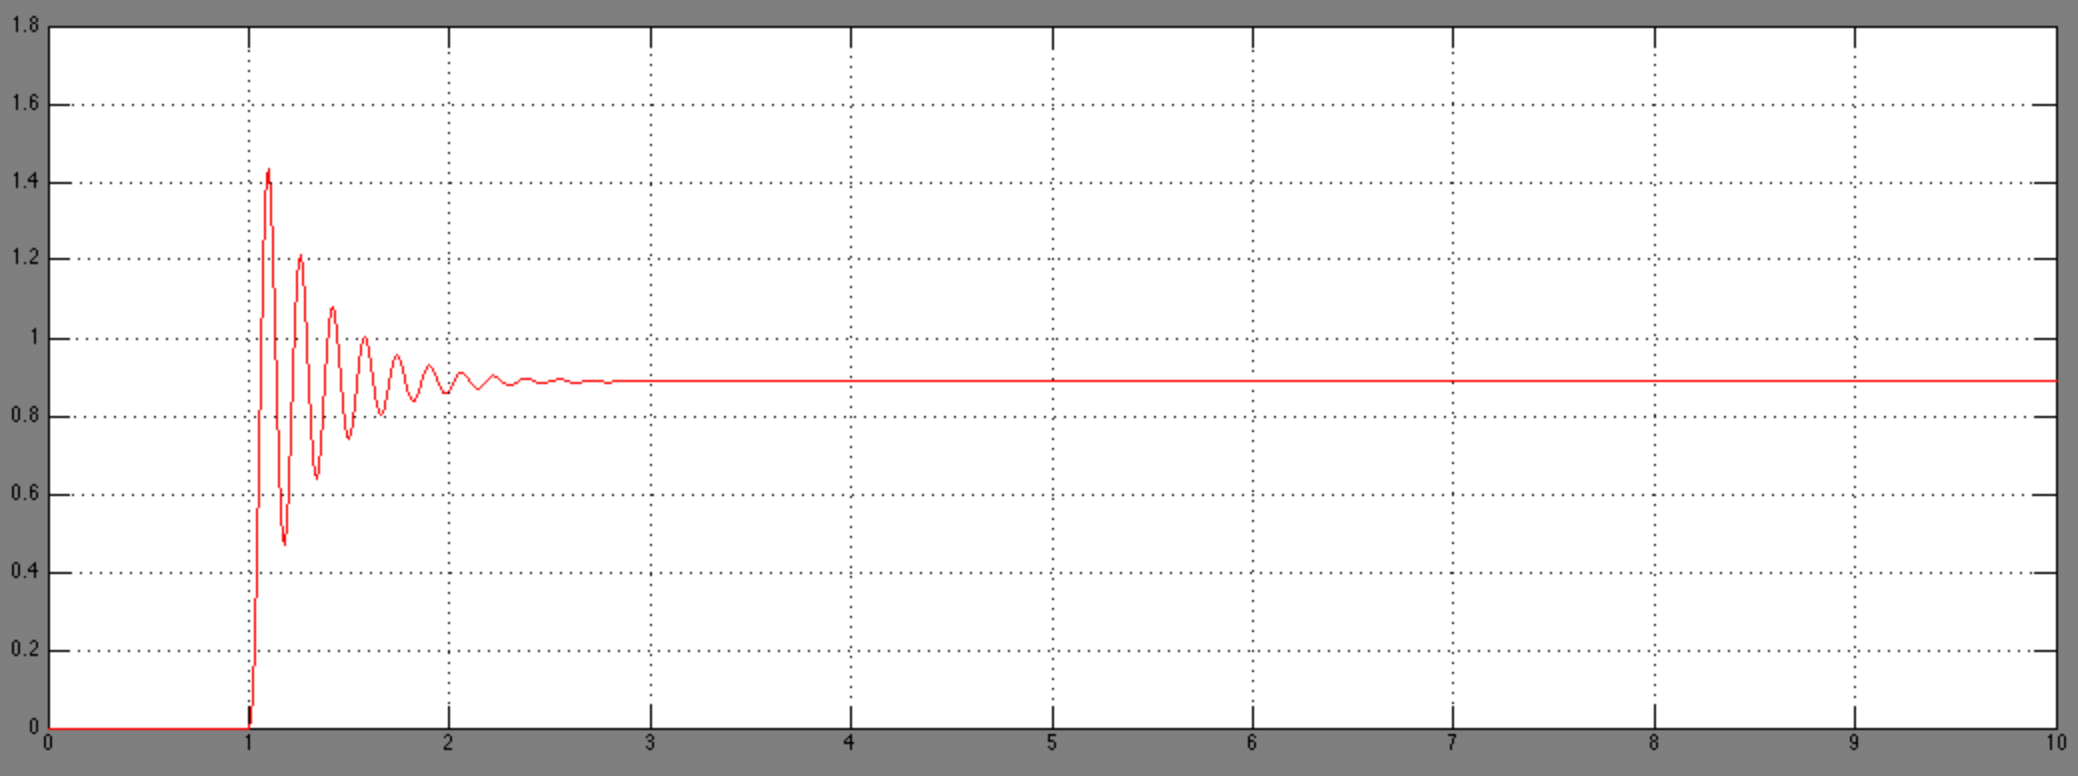
\includegraphics[width = \linewidth]{ki_step0.png}
\caption{step response with $K_I = 0 $}
\floatfoot{Generated using Simulink}
\end{figure}
\FloatBarrier

\begin{figure}[h!]
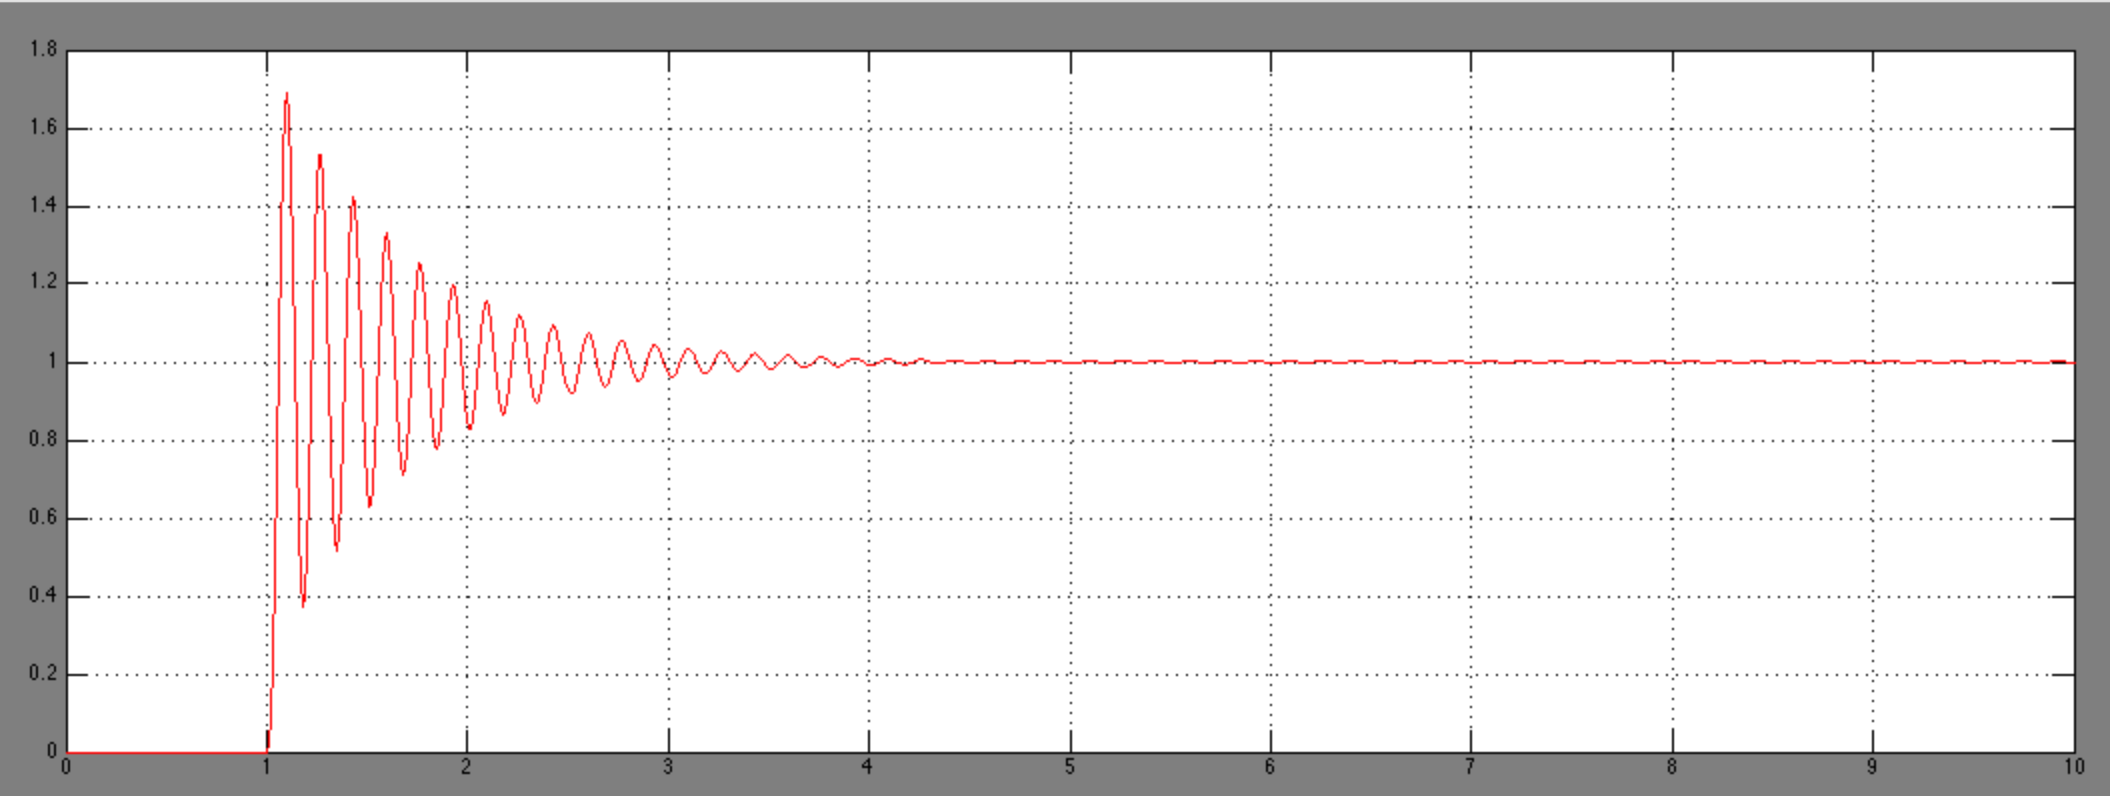
\includegraphics[width = \linewidth]{ki_step.png}
\caption{step response with $K_I$ of 22 }
\floatfoot{Generated using Simulink} 
\end{figure}
\FloatBarrier 


\section{Neutral Stablilty using Simulink} 
I started this section by modelling in Simulink the black box system with the time delay. 
I added the transfer equation and formed a root locus graph. I noticed that it seemd that any value that I chose that stayed to the left  of the real axis and was on the plot would result in a stable system for this function. 
\begin{figure}[h!]
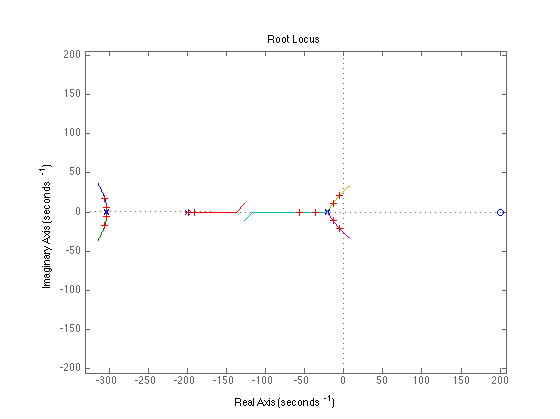
\includegraphics[width = \linewidth]{rlocusnstable.png}
\caption{Time delayed function}
\floatfoot{Generated using Transfer functionl} 
\end{figure}
\FloatBarrier
I noticed the signal was stable at lower values for K, but as long as it was left of the real axis and on the plot I was able to produce a stable graph for K values from .0802 up until 2  
\begin{figure}[h!]
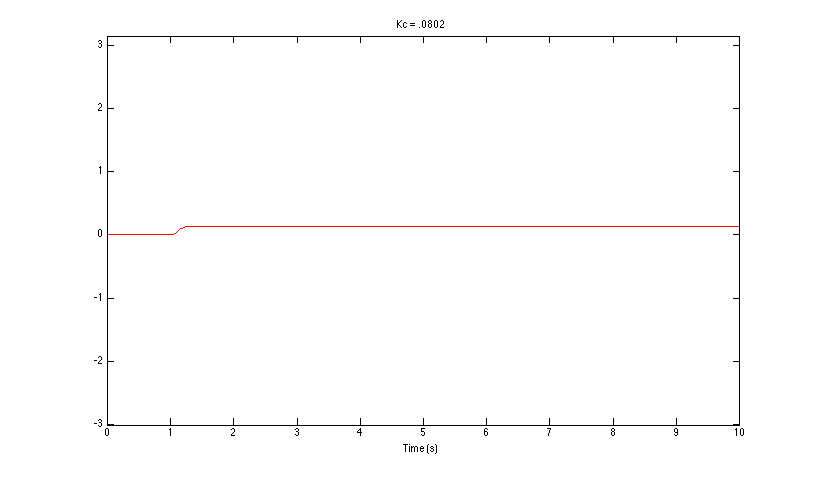
\includegraphics[width = \linewidth]{lownstable.png}
\caption{Time delayed function with K = .0802}
\floatfoot{Generated using Transfer functionl} 
\end{figure}
\FloatBarrier
\begin{figure}[h!]
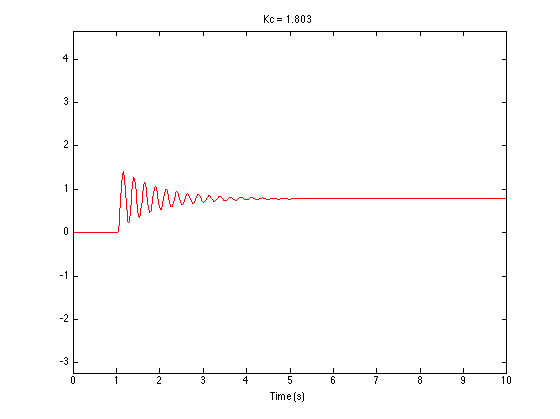
\includegraphics[width = \linewidth]{nunstablelarge.png}
\caption{Time delayed function with K = 1.803}
\floatfoot{Generated using Transfer functionl} 
\end{figure}
\begin{figure}[h!]
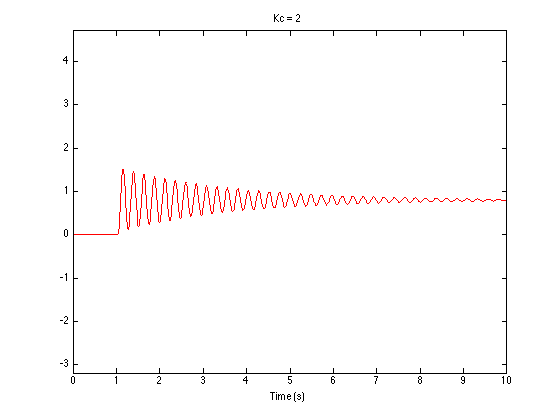
\includegraphics[width = \linewidth]{highnstable.png}
\caption{Time delayed function with K = 2}
\floatfoot{Generated using Transfer functionl} 
\end{figure}
\FloatBarrier


\end{document}
